\documentclass[
  unicode,a4paper,9pt,
  % aspectratio=169,
  xcolor = {dvipsnames,svgnames},
  hyperref ={colorlinks=true,citecolor=Navy,linkcolor=NavyBlue,urlcolor=purple},
  ja=standard,lualatex
]{beamer}
\renewcommand{\baselinestretch}{1.4}

% ---fonts---
\PassOptionsToPackage{quiet}{fontspec}
\usefonttheme{serif}
\mathversion{bold}
\usepackage{luatexja-fontspec}
\setmainfont{TeX Gyre Termes}
\setmainjfont{Noto Sans CJK JP}
% \setmainjfont[BoldFont = HaranoAjiGothic-Regular]{HaranoAjiMincho}
% \setmainjfont[BoldFont = IPAGothic]{IPAMincho}
\setmathrm{Latin Modern Roman}
% \usepackage{newtxmath}

\usepackage{newunicodechar}
\newunicodechar{–}{-}

% ---refer `texdoc xcolor' at the command line---

% ---Display \subsubsection at the Index
% \setcounter{tocdepth}{3}

% ---Setting about the geometry of the document----
% \usepackage{a4wide}
% \pagestyle{empty}

% ---Physics and Math Packages---
\usepackage{amssymb,amsfonts,amsthm,mathtools}
\usepackage{physics,braket,bm,slashed}

% ---underline---
\usepackage[normalem]{ulem}

% ---cancel---
\usepackage{cancel}

% --- surround the texts or equations
\usepackage{fancybox,ascmac}

% ---settings of theorem environment---
\usepackage{amsthm}
\theoremstyle{definition}

% ---settings of proof environment---
\renewcommand{\proofname}{\textbf{証明}}
\renewcommand{\qedsymbol}{$\blacksquare$}

% ---Insert the figure (If insert the `draft' at the option, the process becomes faster.)---
\usepackage{graphicx}
% \usepackage{subcaption}

% ----Add a link to a text---
\usepackage{url,hyperref}
\usepackage{xcolor}

% ---Tikz---
\usepackage{tikz,pgf,pgfplots,circuitikz}
\pgfplotsset{compat=1.15}
\usetikzlibrary{intersections,arrows.meta,angles,calc,3d,decorations.pathmorphing,positioning}

% ---Add the section number to the equation, figure, and table number---
\makeatletter
   \renewcommand{\theequation}{\thesection.\arabic{equation}}
   \@addtoreset{equation}{section}
   
   \renewcommand{\thefigure}{\thesection.\arabic{figure}}
   \@addtoreset{figure}{section}
   
   \renewcommand{\thetable}{\thesection.\arabic{table}}
   \@addtoreset{table}{section}
\makeatother

% ---enumerate---
% \renewcommand{\labelenumi}{$\arabic{enumi}.$}
% \renewcommand{\labelenumii}{$(\arabic{enumii})$}

% ---beamer settings---
\usefonttheme{professionalfonts}
\usecolortheme{seahorse}
\setbeamercolor{structure}{fg=white}
\setbeamercolor{local structure}{fg=red}
\setbeamertemplate{itemize item}[ball]
\setbeamertemplate{enumerate item}[circle]
\setbeamercolor{bibliography entry author}{fg=black}
\setbeamercolor{bibliography item}{fg=black}
\setbeamercolor{alerted text}{fg=RoyalBlue}
\setbeamertemplate{frametitle continuation}{}
\setbeamertemplate{footline}[frame number]
\setbeamertemplate{navigation symbols}{} 
\setbeamersize{text margin left=10pt, text margin right=10pt}

% ---tcolorbox---
\usepackage{tcolorbox}
\tcbuselibrary{theorems}
\tcbuselibrary{raster}
\tcbuselibrary{skins}
\newtcolorbox{bluebox}[2][]{enhanced,
colframe=RoyalBlue!40!white,
colback=RoyalBlue!10!white,
coltitle=black,
drop fuzzy shadow, title={#2}
,#1}
\newtcolorbox{redbox}[2][]{enhanced,
colframe=DarkRed!40!white,
colback=DarkRed!10!white,
coltitle=black,
drop fuzzy shadow, title={#2}
,#1}

% ---tcolorbox---
\usepackage{tcolorbox}
\tcbuselibrary{raster,skins,breakable}
\newtcolorbox{graybox}[1][]{frame empty, colback=black!10!white, sharp corners}

% ---Ignore the Warnings---
\usepackage{silence}
\WarningFilter{latexfont}{Some font shapes}
\WarningFilter{latexfont}{Font shape}
\WarningFilter{latexfont}{Size substitutions}
\ExplSyntaxOn
\msg_redirect_name:nnn{hooks}{generic-deprecated}{none}
\ExplSyntaxOff

% ---Citation on the slides---
\newcommand*{\citefone}[2]{
  \begin{tikzpicture}[remember picture, overlay]
    \node[anchor=north east, align=left] at ($(current page.north east)-(0,0.0)$){
    {\tiny
      \cite{#1}
      #2
    }
    };
  \end{tikzpicture}

  \vspace*{-20pt}
}

\newcommand*{\citeftwo}[4]{
  \begin{tikzpicture}[remember picture, overlay]
    \node[anchor=north east, align=left] at ($(current page.north east)-(0,0.0)$){
    {\tiny
      \cite{#1}
      #2
    }
    \\[-2.4ex]
    {\tiny
      \cite{#3}
      #4
    }
    };
  \end{tikzpicture}

  \vspace*{-20pt}
}

\newcommand*{\citefthree}[6]{
  \begin{tikzpicture}[remember picture, overlay]
    \node[anchor=north east, align=left] at ($(current page.north east)-(0,0.0)$){
    {\tiny
      \cite{#1}
      #2
    }
    \\[-2.4ex]
    {\tiny
      \cite{#3}
      #4
    }
    \\[-2.4ex]
    {\tiny
      \cite{#5}
      #6
    }
    };
  \end{tikzpicture}

  \vspace*{-20pt}
}

\newcommand*{\citefonev}[3]{
  \begin{tikzpicture}[remember picture, overlay]
    \node[anchor=north east, align=left, text width=#3cm] at ($(current page.north east)-(0,0.0)$){
    {{\fontsize{5pt}{0pt}\selectfont
      \cite{#1}
      #2\par}
    }
    };
  \end{tikzpicture}

  \vspace*{-20pt}
}

\newcommand*{\citeftwov}[5]{
  \begin{tikzpicture}[remember picture, overlay]
    \node[anchor=north east, align=left, text width=#5cm] at ($(current page.north east)-(0,0.0)$){
    {{\fontsize{5pt}{0pt}\selectfont
      \cite{#1}
      #2\par}

      {\fontsize{5pt}{0pt}\selectfont
      \cite{#3}
      #4\par}
    }
    };
  \end{tikzpicture}

  \vspace*{-20pt}
}

\newcommand*{\citefthreev}[7]{
  \begin{tikzpicture}[remember picture, overlay]
    \node[anchor=north east, align=left, text width=#7cm] at ($(current page.north east)-(0,0.0)$){
    {{\fontsize{5pt}{0pt}\selectfont
    \cite{#1}
    #2\par}

    {\fontsize{5pt}{0pt}\selectfont
    \cite{#3}
    #4\par}

    {\fontsize{5pt}{0pt}\selectfont
    \cite{#5}
    #6\par}
    }
    };
  \end{tikzpicture}

  \vspace*{-20pt}
}


% ---Title---
\title{
  title
}
\author{
  author
}
\date{Last modified: \today}

\begin{document}

\begin{frame}

  \setbeamertemplate{blocks}[rounded][shadow=true]
  \setbeamercolor{block body}{bg=RoyalBlue!10!white, fg=black}
  \begin{block}{}
    \vspace*{5pt}

    \centering\Large
    Spontaneous R-symmetry breaking in O'Raifeartaigh models
    \\
    \normalsize
    David Shih.
    \\
    \small
    \href{https://doi.org/10.1088/1126-6708/2008/02/091}{JHEP 02 (2008) 091},
    \href{https://arxiv.org/abs/hep-th/0703196}{arXiv:hep-th/0703196}.

    \vspace*{5pt}
  \end{block}

  \vspace*{1cm}

  \begin{center}
    安倍研 M1 宮根一樹\\
    2024 6/20 (木)
  \end{center}

\end{frame}

\nocite{Shih:2007av}

\begin{frame}
  \frametitle{読んだ動機など}
  \citefone{Shih:2007av}{D. Shih, JHEP 02 (2008) 091.}

  \begin{center}
    「現在行っているモジュライ固定の研究に、R対称性の観点から何か言えるかもしれない」
  \end{center}
  というお話があったので、今回は以下の論文を読んできました。

  \begin{figure}
    \centering
    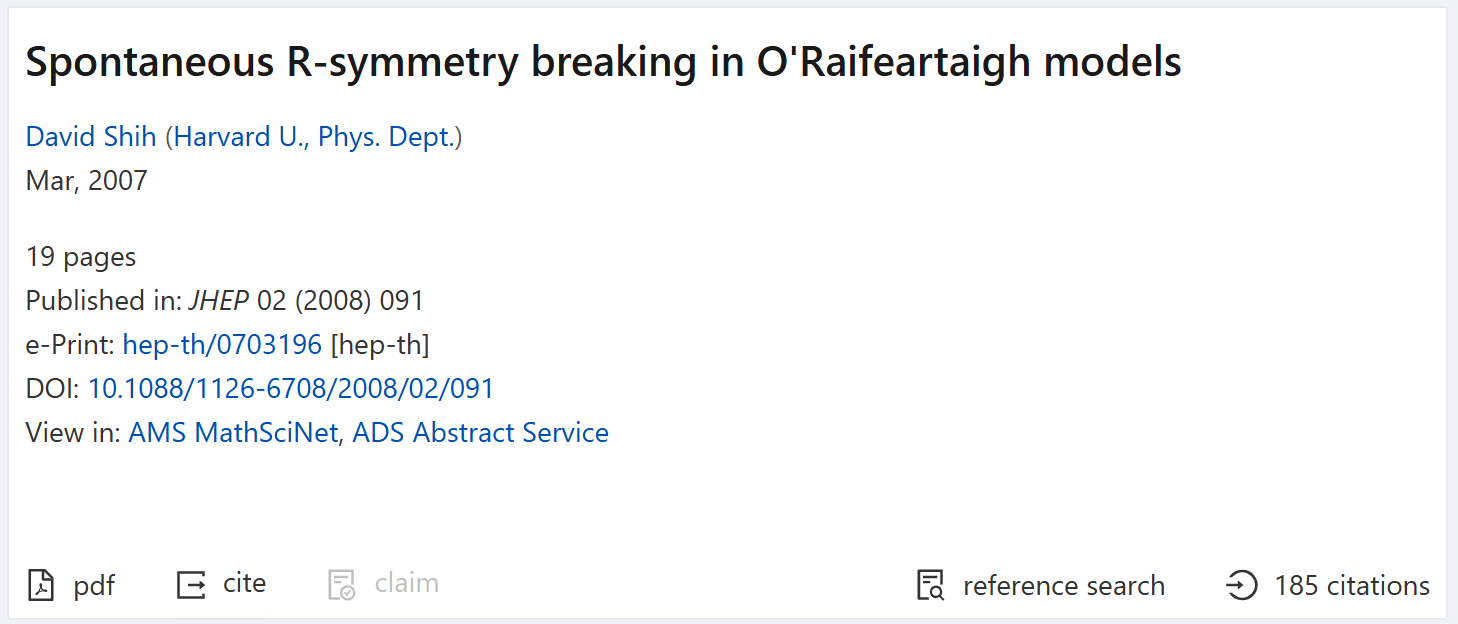
\includegraphics[width=0.8\textwidth]{fig/Shih2007av.PNG}
  \end{figure}

\end{frame}

\begin{frame}
  \frametitle{自発的対称性の破れ}

  $n$個の場$\textcolor{DarkGreen}{\Phi_{i}(x)}$が作るポテンシャル$V(\textcolor{DarkGreen}{\Phi_{1},\cdots,\Phi_{n}})$の極小値に興味がある。

  その極小な点(準安定点)を\textbf{真空}といい、その真空からの揺らぎを考える。
  \begin{equation}
    \textcolor{DarkGreen}{\Phi_{i}}
    =
    \textcolor{RoyalBlue}{\ev*{\Phi_{i}}}+\textcolor{FireBrick}{\tilde{\Phi}_{i}}
    \nonumber
  \end{equation}

\end{frame}

\begin{frame}
  \citefone{Nelson:1993nf}{A. E. Nelson and N. Seiberg, Nucl. Phys. B 416 (1994) 46-62.}
  
  超対称性の破れとR対称性の関連について、Nelson, Seibergらの仕事がある\cite{Nelson:1993nf}。







\end{frame}


\begin{frame}
  \citefone{Nelson:1993nf}{A. E. Nelson and N. Seiberg, Nucl. Phys. B 416 (1994) 46-62.}

  % 今回の論文の立ち位置は?
  









\end{frame}

\section{イントロダクション}

\begin{frame}[plain]
  \huge \secname
\end{frame}

















% --------------------------

\newcounter{Appendix}
\setcounter{Appendix}{\value{framenumber}}
\setcounter{section}{0}
\renewcommand{\thesubsection}{\Alph{subsection}}
\makeatletter
\renewcommand{\theequation}{\thesubsection.\arabic{equation}}
\@addtoreset{equation}{section}

\renewcommand{\thefigure}{\thesubsection.\arabic{figure}}
\@addtoreset{figure}{section}

\renewcommand{\thetable}{\thesubsection.\arabic{table}}
\@addtoreset{table}{section}
\makeatother

\section{付録}

\begin{frame}[plain]
  \frametitle{\ }
  \huge \secname
\end{frame}

\subsection{目次}

\begin{frame}[plain,allowframebreaks]{\thesubsection. \subsecname}
  \tableofcontents
\end{frame}



% --------------------------

\section{参考文献}
\begin{frame}[plain,allowframebreaks]{\secname}

  \scriptsize
  \beamertemplatetextbibitems
  \bibliographystyle{ytphys}
  \bibliography{ref}

\end{frame}

\setcounter{framenumber}{\value{Appendix}}
\end{document}
